\chapter{Hypothesis Testing}

In this chapter, we will design comprehensive experiments to probe the proposed hypotheses detailed in Section \ref{sec:researchquestions}. Some of the hypotheses have already found compelling answers in the existing research literature, as reviewed in Section \ref{chp:RelatedWork}. For those hypotheses yet unaddressed, the model, which was formulated and described in Section \ref{sec:model}, will be employed for rigorous evaluation. The datasets that will be utilized for this evaluation process are referenced in Section \ref{subsec:dataset}. 

With the stated hypotheses, we aim to extend the envelope of existing understanding and contribute novel insights into the domain of image fusion. We expect that the carefully designed experimental procedure will offer a robust platform to scrutinize these hypotheses, shed light on the latent aspects, and help us further refine our model's capability and performance.

The untested or unanswered hypotheses, which still pose intriguing questions and challenges to our research pursuit, can be articulated as follows:

\begin{list}{}{}
    \item \textbf{Hypothesis I-1}: The new loss function, which emphasizes the similarity between both the visible band input and the infrared image input, will result in more informative and meaningful fused images compared to using Structural Similarity Metric (SSIM) as the guiding criterion.

    \item \textbf{Hypothesis II-1}: The combination of Transformer-based models and the new loss function will significantly improve night vision enhancement, medical imaging, and surveillance tasks, allowing for better object detection, classification, and tracking in challenging lighting conditions.
    
    \item \textbf{Hypothesis II-2}: The proposed transformer based approach will achieve a better balance between quantitative and qualitative performance in image fusion, overcoming the compromise between the two that is often observed in traditional deep learning methods.
    
    \item \textbf{Hypothesis II-3}: The proposed approach will demonstrate computational efficiency, making it suitable for real-time applications, such as video surveillance and live medical imaging, without sacrificing the quality of the fused images.
    
    \item \textbf{Hypothesis II-4}: The limitations and challenges associated with implementing Transformer-based image fusion techniques can be mitigated through proper model tuning, regularization, and architecture adjustments, leading to improved overall performance.
    
    \item \textbf{Hypothesis I-2}: The proposed approach will surpass existing state-of-the-art image fusion methods in terms of visual quality, providing more detailed, sharper, and visually appealing fused images.
    
\end{list}

Each of these proposed hypotheses will be systematically evaluated in subsequent sections. The hypotheses concerning the significance of transformers and the role of global context will be scrutinized in Section \ref{sec:study1}. On the other hand, the hypotheses associated with the loss function's applicability and effectiveness will be put to rigorous examination in Section \ref{sec:study2}. In essence, we seek to undertake a meticulous exploration of each hypothesis to validate their tenability within the theoretical and empirical constructs of our research. As you may see from the above list \textbf{Hypothesis Hypothesis I-3} will be remained for further studies.

\section{Study I: New Loss Function Proposal}\label{sec:study2}

The first part of our research, \textit{Study I}, delves further into the specifics of our model's novel aspects and their impact, particularly focusing on the new loss function and the expanded potential applications of our approach. We anticipate the following outcomes based on these hypotheses:

\begin{itemize}
    \item \textbf{Hypothesis I-1}: The new loss function, which emphasizes the similarity between both the visible band input and the infrared image input, will result in more informative and meaningful fused images compared to using Structural Similarity Metric (SSIM) as the guiding criterion.
    
    \item \textbf{Hypothesis I-2}: The proposed approach will surpass existing state-of-the-art image fusion methods in terms of visual quality, providing more detailed, sharper, and visually appealing fused images.
    
    \item \textbf{Hypothesis Hypothesis I-3}: The combination of Transformer-based models and the new loss function will pave the way for innovative applications in image fusion, such as advanced medical diagnostics, autonomous driving, and precision agriculture.
\end{itemize}

We focus on our new loss function in \textbf{Hypothesis I-1}, which plays a pivotal role in our approach. This novel loss function emphasizes the similarity between both the visual and infrared image inputs, which we anticipate will result in fused images that are more informative and meaningful. To validate this, we will compare our fused images with those obtained using other guiding criteria, such as the Structural Similarity Metric (SSIM).

\textbf{Hypothesis I-2} asserts that our approach will outperform existing state-of-the-art image fusion techniques in terms of visual quality. This will be assessed through a comparative analysis of our approach and other leading methods. A combination of both objective and subjective evaluations will be used. Objective evaluations will focus on statistical measures of image quality, while subjective evaluations will be based on human visual perception of the fused images' clarity, sharpness, and overall visual appeal.

Through this multi-pronged experimental design, we aim to thoroughly validate our hypotheses, contributing significantly to the growing body of knowledge in transformer-based image fusion techniques. Our results could illuminate new pathways for the application of these models, extending their impact beyond traditional domains.

\subsection{Method To Test Hypothesis I-1: Loss Function Comparison} \label{subsec:met2}


\textbf{Hypothesis I-1} proposes that our novel loss function, which emphasizes the similarity between both the visible band input and the infrared image input, will result in more informative and meaningful fused images compared to using the Structural Similarity Metric (SSIM) as the guiding criterion. To validate this hypothesis, we will take the following steps:

\begin{itemize}

    \item \textit{Loss Function Implementation:} Implement the proposed loss function in the model. This loss function will be designed to stress the preservation of significant features from both the visible band and the infrared image inputs.

    \item \textit{Training with Different Loss Functions:} Train multiple versions of the proposed model using different loss functions. One version will utilize the traditional SSIM loss function, and the other will employ the newly proposed loss function. All other parameters and settings will be kept consistent to ensure a fair comparison.

    \item \textit{Visual Evaluation:} Conduct a qualitative evaluation of the fused images produced by both models. This includes assessing the preservation of details from the source images, the contrast, sharpness, and overall perceptual quality of the fused images.

    \item \textit{Quantitative Evaluation:} Quantitatively compare the performance of both models by computing metrics like p$SSIM$, and mutual information for the fused images.

\end{itemize}

By comparing the quality and information retention in the fused images produced using the two different loss functions, we can assess the validity of Hypothesis I-1.

\subsection{Test Results Related To Hypothesis I-1: Loss Function Comparison} \label{subsec:met2res}

As we discussed through the Section \ref{subsec:met2}, on how to test hypothesis 2. We have defined the $L_{fuse}$ as in Eq. \ref{eq:fuseloss}. During the experiment, we have compared the model performance with both $L_{fuse}$ and $L_{ae}$ at Eq \ref{eq:aeloss}. The Figure \ref{fig:ch5:met2} compares the results qualitatively.

\begin{table}[htbp]
    \centering
    \caption{Hypothesis I-1 Results: Loss Function Comparison}
    \label{tab:ch5:met2}
    \begin{tabular}{|l|l|l|l|l|}
        \hline
        \textbf{Folder} & \textbf{Entropy\cite{roberts2008assessment}$\uparrow$ } & \textbf{SCD\cite{aslantas2015new}$\downarrow$} & \textbf{MI\cite{qu2002information}$\uparrow$} & \textbf{SSIM\cite{ma2015perceptual}$\uparrow$} \\ \hline
        Proposed $L_{fuse}$ in Eq\ref{eq:fuseloss}            & 4.536                & \textbf{5.433}       & \textbf{1.591}           & \textbf{0.884}             \\ \hline
        $L_{ae}$ as $L_{fuse}$ Exp            & 4.559                & 6.466       & 0.552           & 0.879             \\ \hline
        RFN-Nest\cite{li2021rfn}            & \textbf{4.729}                & 7.062       & 0.602           & 0.541             \\ \hline
    \end{tabular}
\end{table}

Upon examining Figure \ref{fig:ch5:met2} and Table \ref{tab:ch5:met2}, it becomes evident that the newly proposed loss function demonstrates a commendable ability to produce both qualitative and quantitative results. Given that both loss functions are expressed in relation to the \(SSIM(.)\) metric, it is more coherent to investigate other metrics when identical \(SSIM()\) values are observed. For the sake of a comprehensive comparison, it is pertinent to mention that the RFN-Nest results have been included. The model employing the loss function labeled as "\(L_{ae}\) as \(L_{fuse}\) Exp" has the potential to achieve an elevated SSIM score, as cited in \cite{ma2015perceptual}. In scenarios where this occurs, the image quality diminishes, eventually matching the quality of the input visual image. Theoretically, this process could lead to an impeccable fusion, signified by \(SSIM(.) = 1\). Given that \(SSIM(X,Y) \iff X=Y\), such a scenario would result in the direct replication of the input visual band image in the output. Notably, when evaluated at nearly identical \(SSIM(/)\) scores, the loss function proposed in Eq. \ref{eq:fuseloss} showcases superior performance compared to the conventionally adopted loss function detailed in Eq. \ref{eq:aeloss}.\

\begin{figure}[htbp]
    \centering
    \begin{subfigure}[b]{\textwidth}
        \includegraphics[width=0.32\textwidth, height=0.15\textheight]{images/ch5/vis/20.png}
        \includegraphics[width=0.32\textwidth, height=0.15\textheight]{images/ch5/vis/12.png}
        \includegraphics[width=0.32\textwidth, height=0.15\textheight]{images/ch5/vis/02.png}
        \caption{Visual Band Images}
        \label{fig:ch5:met2:vis}
    \end{subfigure}
    \vspace{0.01cm}
    \begin{subfigure}[b]{\textwidth}
        \includegraphics[width=0.32\textwidth, height=0.15\textheight]{images/ch5/ir/20.png}
        \includegraphics[width=0.32\textwidth, height=0.15\textheight]{images/ch5/ir/12.png}
        \includegraphics[width=0.32\textwidth, height=0.15\textheight]{images/ch5/ir/02.png}
        \caption{Infrared Band Images}
        \label{fig:ch5:met2:ir}
    \end{subfigure}
    \vspace{0.01cm}
    \begin{subfigure}[b]{\textwidth}
        \includegraphics[width=0.32\textwidth, height=0.15\textheight]{images/ch5/ours/20.jpg}
        \includegraphics[width=0.32\textwidth, height=0.15\textheight]{images/ch5/ours/12.jpg}
        \includegraphics[width=0.32\textwidth, height=0.15\textheight]{images/ch5/ours/02.jpg}
        \caption{Model With New $L_{fuse}$ Loss Output Images}
        \label{fig:ch5:met2:ours}
    \end{subfigure}
    \vspace{0.01cm}
    \begin{subfigure}[b]{\textwidth}
        \includegraphics[width=0.32\textwidth, height=0.15\textheight]{images/ch5/sameLoss/20.png}
        \includegraphics[width=0.32\textwidth, height=0.15\textheight]{images/ch5/sameLoss/12.png}
        \includegraphics[width=0.32\textwidth, height=0.15\textheight]{images/ch5/sameLoss/02.png}
        \caption{Model With $ L_{fuse} = L_{ae}$ Loss Output Images}
        \label{fig:ch5:met2:sameLoss}
    \end{subfigure}
    \caption{Hypothesis I-1 Results: Loss Function Comparison}
    \label{fig:ch5:met2}
\end{figure}

Building on the aforementioned observations, it's worth emphasizing the significance of the innovative approach embodied by the newly proposed loss function. The consistent performance, as underlined by the results in Figure \ref{fig:ch5:met2} and Table \ref{tab:ch5:met2}, serves as a testament to its potential in enhancing image processing techniques. The inclusion of RFN-Nest results not only ensures a comprehensive assessment but also underscores the comparative advantages of our proposed methodology. The ability of a model to match or even outperform traditional standards, especially in terms of the \(SSIM(.)\) metric, sets a new benchmark for future research. The direct correspondence between \(SSIM(X,Y)\) and the output mirroring the input visual band image opens up avenues for further exploration, particularly in applications where image fidelity is paramount. As we push the boundaries of existing loss functions, the results from Eq. \ref{eq:fuseloss} offer promising insights, potentially paving the way for advancements in image fusion and related fields.

\subsection{Method To Test Hypothesis I-2: Comparison with SoTAHypothesis I-2} \label{subsec:met9}

\textbf{Hypothesis I-2} posits that the proposed approach will surpass existing state-of-the-art image fusion methods in terms of visual quality, providing more detailed, sharper, and visually appealing fused images. To evaluate the validity of this hypothesis, the following steps will be followed:

\begin{itemize}
    \item \textit{Selection of Benchmark Models:} Choose a set of state-of-the-art image fusion methods as benchmarks. These models should represent the current best performance in image fusion tasks.

    \item \textit{Training and Fusion:} Train the proposed model and each of the benchmark models on the same dataset. Perform image fusion using each of these trained models.

    \item \textit{Visual Comparison:} Conduct a visual comparison of the fused images produced by the proposed model and each of the benchmark models. This qualitative assessment will involve judging the sharpness, clarity, and detail preservation in the fused images.

    \item \textit{Quantitative Comparison:} Use established image quality metrics such as PSNR, SSIM, and mutual information to provide a quantitative comparison of the quality of fused images produced by each model.

\end{itemize}


By analyzing the results from the visual, human, and quantitative evaluations, we can infer whether our proposed approach indeed outperforms the current state-of-the-art methods in terms of visual quality of the fused images, thus verifying Hypothesis I-2.

\subsection{Test Results Related To Hypothesis I-2: Comparison with SoTA} \label{subsec:met9res}

In the following section, we plan to compare our model with leading image fusion methods. We'll evaluate them based on visual quality and the quantitative metrics outlined in Section \ref{subsec:metrics}. As highlighted in Section \ref{chp:RelatedWork}, current top methods include transformer-based techniques like M3FD\cite{liu2022target} and IFT\cite{vs2022image}, GAN-based approaches such as DenseFuse\cite{li2019infrared} and SwinFusion\cite{ma2022swinfusion}, and the autoencoder method RFN-Nest\cite{li2021rfn}. Our goal is to provide a clear and thorough comparison to understand the strengths and limitations of each method in the field of image fusion.

\begin{table}[htbp]
    \centering
    \caption{Hypothesis I-2 Results: Comparison with SoTA}
    \label{tab:ch5:met8}
    \begin{tabular}{|l|l|l|l|l|}
        \hline
        \textbf{Method} & \textbf{Entropy\cite{roberts2008assessment}$\uparrow$ } & \textbf{SCD\cite{aslantas2015new}$\downarrow$} & \textbf{MI\cite{qu2002information}$\uparrow$} & \textbf{SSIM\cite{ma2015perceptual}$\uparrow$} \\ \hline
        Ours            & 4.536                & \textbf{5.433}       & \textbf{1.591}           &\textbf{0.884}             \\ \hline
        SwinFusion\cite{ma2022swinfusion}           & 4.605                & 6.760       & 0.804           & 0.690             \\ \hline
        M3FD\cite{liu2022target}           & 4.625                & 6.858       & 0.742           & 0.659             \\ \hline
        IFT\cite{vs2022image}           & 4.644                & 6.864       & 0.684           & 0.630             \\ \hline
        DenseFuse\cite{li2019infrared}           & 4.724                & 6.455       & 0.853           & 0.588             \\ \hline
        RFN-Nest\cite{li2021rfn}            & \textbf{4.729}                & 7.062       & 0.602           & 0.541             \\ \hline
    \end{tabular}
\end{table}

\begin{figure}[htbp]
    \centering
    \begin{subfigure}[b]{\textwidth}
        \includegraphics[width=0.32\textwidth, height=0.15\textheight]{images/ch5/vis/20.png}
        \includegraphics[width=0.32\textwidth, height=0.15\textheight]{images/ch5/vis/12.png}
        \includegraphics[width=0.32\textwidth, height=0.15\textheight]{images/ch5/vis/02.png}
        \caption{Visual Band Images}
        \label{fig:ch5:met9:vis}
    \end{subfigure}
    \vspace{0.01cm}
    \begin{subfigure}[b]{\textwidth}
        \includegraphics[width=0.32\textwidth, height=0.15\textheight]{images/ch5/ir/20.png}
        \includegraphics[width=0.32\textwidth, height=0.15\textheight]{images/ch5/ir/12.png}
        \includegraphics[width=0.32\textwidth, height=0.15\textheight]{images/ch5/ir/02.png}
        \caption{Infrared Band Images}
        \label{fig:ch5:met9:ir}
    \end{subfigure}
    \vspace{0.01cm}
    \begin{subfigure}[b]{\textwidth}
        \includegraphics[width=0.32\textwidth, height=0.15\textheight]{images/ch5/ours/20.jpg}
        \includegraphics[width=0.32\textwidth, height=0.15\textheight]{images/ch5/ours/12.jpg}
        \includegraphics[width=0.32\textwidth, height=0.15\textheight]{images/ch5/ours/02.jpg}
        \caption{Our Output Images}
        \label{fig:ch5:met9:ours}
    \end{subfigure}
    \vspace{0.01cm}
    \begin{subfigure}[b]{\textwidth}
        \includegraphics[width=0.32\textwidth, height=0.15\textheight]{images/ch5/swinFusion/20.jpg}
        \includegraphics[width=0.32\textwidth, height=0.15\textheight]{images/ch5/swinFusion/12.jpg}
        \includegraphics[width=0.32\textwidth, height=0.15\textheight]{images/ch5/swinFusion/02.jpg}
        \caption{SwinFusion\cite{ma2022swinfusion} Output Images}
        \label{fig:ch5:met9:swin}
    \end{subfigure}
    \caption{Hypothesis I-2 Results: Comparison with SoTA}
    \label{fig:ch5:met4}
\end{figure}

\begin{figure}[htbp]
    \centering
    \begin{subfigure}[b]{\textwidth}
        \includegraphics[width=0.32\textwidth, height=0.15\textheight]{images/ch5/m3fd/20.jpg}
        \includegraphics[width=0.32\textwidth, height=0.15\textheight]{images/ch5/m3fd/12.jpg}
        \includegraphics[width=0.32\textwidth, height=0.15\textheight]{images/ch5/m3fd/02.jpg}
        \caption{M3FD\cite{liu2022target} Output Images}
        \label{fig:ch5:met9:m3fd}
    \end{subfigure}
    \vspace{0.01cm}
    \begin{subfigure}[b]{\textwidth}
        \includegraphics[width=0.32\textwidth, height=0.15\textheight]{images/ch5/swinFusion/20.jpg}
        \includegraphics[width=0.32\textwidth, height=0.15\textheight]{images/ch5/swinFusion/12.jpg}
        \includegraphics[width=0.32\textwidth, height=0.15\textheight]{images/ch5/swinFusion/02.jpg}
        \caption{IFT\cite{vs2022image} Output Images}
        \label{fig:ch5:met9:ift}
    \end{subfigure}
    \vspace{0.01cm}
    \begin{subfigure}[b]{\textwidth}
        \includegraphics[width=0.32\textwidth, height=0.15\textheight]{images/ch5/rfn/20.png}
        \includegraphics[width=0.32\textwidth, height=0.15\textheight]{images/ch5/rfn/12.png}
        \includegraphics[width=0.32\textwidth, height=0.15\textheight]{images/ch5/rfn/02.png}
        \caption{RFN-Nest\cite{li2021rfn} Output Images}
        \label{fig:ch5:met9:rfn}
    \end{subfigure}
    \vspace{0.01cm}
    \begin{subfigure}[b]{\textwidth}
        \includegraphics[width=0.32\textwidth, height=0.15\textheight]{images/ch5/denseFuse/20.png}
        \includegraphics[width=0.32\textwidth, height=0.15\textheight]{images/ch5/denseFuse/12.png}
        \includegraphics[width=0.32\textwidth, height=0.15\textheight]{images/ch5/denseFuse/02.png}
        \caption{DenseFuse\cite{li2019infrared} Output Images}
        \label{fig:ch5:met9:densefuse}
    \end{subfigure}
    \caption{Hypothesis I-2 Results: Comparison with SoTA cont'd}
\end{figure}

Upon a qualitative assessment of Figure \ref{fig:ch5:met5}, several observations come to the fore. The first column distinctly showcases the imaging of a soldier amidst smoke, and this rendition, with its meticulous portrayal of the surrounding details, stands qualitatively superior to its counterparts. A similar superiority can be discerned in the second column, where the depiction of the man concealed behind the tree is accentuated by the intricate details of the tree's broader context, setting it apart from other state-of-the-art methods presented.

The final column further underscores the prowess of our method. Here, one can distinctly discern the brand name on a shop awning and identify pedestrians on the street, all the while maintaining the fidelity of details from the original visual band images.

Turning our attention to Table \ref{tab:ch5:met8}, it becomes evident that our method eclipses others in performance across almost all metrics. The sole exception is the \(Entropy\cite{roberts2008assessment}\) metric. It's worth noting that entropy gauges the degree to which pixel values in an image are non-redundant. Consequently, original infrared images, as depicted in Figure \ref{fig:ch5:met2:ir}, would naturally register the highest entropy scores. This distinction provides a nuanced understanding of where and how our method stands in relation to others in the domain. 

\section{Study II: A Unique Transformer Based Fusion Strategy}\label{sec:study1}

Our research aims to explore the application of transformer-based models in the context of visual and infrared image fusion, with an emphasis on utilizing autoencoders for feature extraction and representation learning. This study is rooted in the following hypotheses:

\begin{itemize}
    \item \textbf{Hypothesis II-1}: The combination of Transformer-based models and the new loss function will significantly improve night vision enhancement, medical imaging, and surveillance tasks, allowing for better object detection, classification, and tracking in challenging lighting conditions.
    
    \item \textbf{Hypothesis II-2}: The proposed transformer-based approach will achieve a better balance between quantitative and qualitative performance in image fusion, overcoming the compromise between the two that is often observed in traditional deep learning methods.
    
    \item \textbf{Hypothesis II-3}: The proposed approach will demonstrate computational efficiency, making it suitable for real-time applications, such as video surveillance and live medical imaging, without sacrificing the quality of the fused images.
    
    \item \textbf{Hypothesis II-4}: The limitations and challenges associated with implementing Transformer-based image fusion techniques can be mitigated through proper model tuning, regularization, and architecture adjustments, leading to improved overall performance.
\end{itemize}

Our proposed approach builds upon the use of an autoencoder to extract salient features from both visual and infrared images. These feature maps are then fused using a transformer-based approach, incorporating the strengths of both convolutional neural networks and transformer models. The fused features are then reconstructed into a final coherent representation using a single decoder. This architecture has been designed to address the challenges associated with implementing transformer-based image fusion techniques and aims to balance performance and computational efficiency.

We designed experiments to empirically evaluate these hypotheses. The experiments were performed using the TNO dataset, which provides a diverse collection of visual and infrared images, making it ideal for image fusion tasks. Each hypothesis corresponds to a specific aspect of our model's design or objective and guided the development of specific experiments:

For \textbf{Hypothesis II-1}, we will evaluate the performance of our model on various tasks such as object detection, classification, and tracking under challenging lighting conditions. We will compare these results with other state-of-the-art models to ascertain the effectiveness of our approach.

In relation to \textbf{Hypothesis II-2}, we will assess the qualitative and quantitative performance of our image fusion model. The quantitative analysis will involve measuring metrics such as Peak Signal-to-Noise Ratio (PSNR), Structural Similarity Index Measure (SSIM), and Fusion Quality Index (FQI). The qualitative analysis, on the other hand, will involve visual assessments and comparisons with other models.

\textbf{Hypothesis II-3} will be evaluated through measuring the computational efficiency of our model in terms of runtime and memory usage during both training and inference. We will also assess the quality of the fused images to ensure that efficiency gains do not come at the expense of fusion quality.

Finally, in testing \textbf{Hypothesis II-4}, we will investigate the effects of various model tuning strategies, regularization techniques, and architecture adjustments on the performance of our transformer-based image fusion model. We expect these techniques to help mitigate some of the limitations and challenges associated with implementing transformer-based image fusion techniques.

The results of these experiments will provide valuable insights into the effectiveness and efficiency of transformer-based image fusion techniques, advancing our understanding and potentially setting the stage for future work in this exciting area.

\subsection{Method To Test HypothesisHypothesis II-1: Night Vision Enhancement} \label{subsec:met4}

\textbf{Hypothesis II-1} postulates that the combination of Transformer-based models and the new loss function will significantly improve task performances such as night vision enhancement, medical imaging, and surveillance tasks, allowing for better object detection, classification, and tracking in challenging lighting conditions. To test this hypothesis, we will adopt a multi-stage evaluation approach, drawing from both qualitative and quantitative assessment methods.

\begin{itemize}
    \item \textit{Dataset Preparation:} We will use a diverse range of images from the TNO dataset, which includes both visual and infrared images under various challenging lighting conditions. The dataset will be divided into a training set and a testing set to ensure the robustness of our model.
    \item \textit{Model Training:} The Transformer-based image fusion model will be trained on the training set, with the new loss function serving as the guiding criterion for the training process. The model's parameters will be optimized iteratively to minimize the loss function.
    \item \textit{Evaluation on Night Vision Enhancement:} To test the model's capability for night vision enhancement, we will use the testing set to create fused images under low-light conditions. The quality of these fused images will be evaluated qualitatively through visual inspection and quantitatively using various image quality metrics stated in Section \ref{subsec:Benchmarking} and \ref{subsec:metrics} such as Structural Similarity Index Metric (SSIM).
    \item \textit{Evaluation on TNO:} We will similarly evaluate the model's performance on TNO dataset. The resultant images will be assessed for their clarity and detail. For surveillance tasks, we will specifically look at how well the model improves object detection.
    \item \textit{Comparison with Baseline Methods:} Finally, we will compare the performance of our model with existing state-of-the-art methods in image fusion. The comparison will be based on both the quality of the fused images and the improvement in object detection, classification, and tracking.
\end{itemize}

The outcome of this evaluation should provide robust evidence regarding the effectiveness of our Transformer-based model and the new loss function in enhancing night vision, and improving medical imaging and surveillance tasks.

\subsection{Test Results Related To Hypothesis II-1: Night Vision Enhancement} \label{subsec:met4res}

In the discussion presented in Section \ref{subsec:met4}, we elucidated the process of training our proposed model utilizing a novel loss function specifically designed for our research objectives. Our primary focus was to enhance the model's capability to handle intricate challenges presented by certain datasets.

To validate the efficacy of our model, we employed the TNO dataset. This dataset is particularly characterized by its challenging scenarios, predominantly encompassing nocturnal settings and other low-light situations. Such conditions are known to test the robustness and adaptability of many computational models, making the TNO dataset an apt choice for our evaluation.

Our evaluation didn't just stop at assessing our model's performance. It was imperative to juxtapose our methods with existing state-of-the-art (SoTA) techniques. By drawing comparisons with contemporary methods in SoTA, we aimed to establish a comprehensive understanding of where our approach stands in the broader landscape of the field. Such comparative analyses are pivotal in highlighting the potential advantages of our technique and identifying areas that might require further refinement.

\begin{figure}[htbp]
    \centering
    \begin{subfigure}[b]{\textwidth}
        \includegraphics[width=0.32\textwidth, height=0.15\textheight]{images/ch5/vis/02.png}
        \includegraphics[width=0.32\textwidth, height=0.15\textheight]{images/ch5/vis/07.png}
        \includegraphics[width=0.32\textwidth, height=0.15\textheight]{images/ch5/vis/11.png}
        \caption{Visual Band Images}
        \label{fig:ch5:met4:vis}
    \end{subfigure}
    \vspace{0.01cm}
    \begin{subfigure}[b]{\textwidth}
        \includegraphics[width=0.32\textwidth, height=0.15\textheight]{images/ch5/ir/02.png}
        \includegraphics[width=0.32\textwidth, height=0.15\textheight]{images/ch5/ir/07.png}
        \includegraphics[width=0.32\textwidth, height=0.15\textheight]{images/ch5/ir/11.png}
        \caption{Infrared Band Images}
        \label{fig:ch5:met4:ir}
    \end{subfigure}
    \vspace{0.01cm}
    \begin{subfigure}[b]{\textwidth}
        \includegraphics[width=0.32\textwidth, height=0.15\textheight]{images/ch5/ours/02.jpg}
        \includegraphics[width=0.32\textwidth, height=0.15\textheight]{images/ch5/ours/07.jpg}
        \includegraphics[width=0.32\textwidth, height=0.15\textheight]{images/ch5/ours/11.jpg}
        \caption{Our Output Images}
        \label{fig:ch5:met4:ours}
    \end{subfigure}
    \vspace{0.01cm}
    \begin{subfigure}[b]{\textwidth}
        \includegraphics[width=0.32\textwidth, height=0.15\textheight]{images/ch5/swinFusion/02.jpg}
        \includegraphics[width=0.32\textwidth, height=0.15\textheight]{images/ch5/swinFusion/07.jpg}
        \includegraphics[width=0.32\textwidth, height=0.15\textheight]{images/ch5/swinFusion/11.jpg}
        \caption{SwinFusion\cite{ma2022swinfusion}Output Images}
        \label{fig:ch5:met4:swin}
    \end{subfigure}
    \caption{Hypothesis II-1 Results: Night Vision Enhancement}
    \label{fig:ch5:met4}
\end{figure}

\begin{figure}[htbp]
    \centering
    \begin{subfigure}[b]{\textwidth}
        \includegraphics[width=0.32\textwidth, height=0.15\textheight]{images/ch5/m3fd/02.jpg}
        \includegraphics[width=0.32\textwidth, height=0.15\textheight]{images/ch5/m3fd/07.jpg}
        \includegraphics[width=0.32\textwidth, height=0.15\textheight]{images/ch5/m3fd/11.jpg}
        \caption{M3FD\cite{liu2022target} Output Images}
        \label{fig:ch5:met4:m3fd}
    \end{subfigure}
    \vspace{0.01cm}
    \begin{subfigure}[b]{\textwidth}
        \includegraphics[width=0.32\textwidth, height=0.15\textheight]{images/ch5/swinFusion/02.jpg}
        \includegraphics[width=0.32\textwidth, height=0.15\textheight]{images/ch5/swinFusion/07.jpg}
        \includegraphics[width=0.32\textwidth, height=0.15\textheight]{images/ch5/swinFusion/11.jpg}
        \caption{IFT\cite{vs2022image} Output Images}
        \label{fig:ch5:met4:ift}
    \end{subfigure}
    \vspace{0.01cm}
    \begin{subfigure}[b]{\textwidth}
        \includegraphics[width=0.32\textwidth, height=0.15\textheight]{images/ch5/rfn/02.png}
        \includegraphics[width=0.32\textwidth, height=0.15\textheight]{images/ch5/rfn/07.png}
        \includegraphics[width=0.32\textwidth, height=0.15\textheight]{images/ch5/rfn/11.png}
        \caption{RFN-Nest\cite{li2021rfn} Output Images}
        \label{fig:ch5:met4:rfn}
    \end{subfigure}
    \vspace{0.01cm}
    \begin{subfigure}[b]{\textwidth}
        \includegraphics[width=0.32\textwidth, height=0.15\textheight]{images/ch5/denseFuse/02.png}
        \includegraphics[width=0.32\textwidth, height=0.15\textheight]{images/ch5/denseFuse/07.png}
        \includegraphics[width=0.32\textwidth, height=0.15\textheight]{images/ch5/denseFuse/11.png}
        \caption{DenseFuse\cite{li2019infrared} Output Images}
        \label{fig:ch5:met4:densefuse}
    \end{subfigure}
    \caption{Hypothesis II-1 Results: Night Vision Enhancement c`ont'd}
\end{figure}

From Figure \ref{fig:ch5:met4}, the first column showcases an instance of night vision imagery. This particular example serves as a suitable representation for illustrating long-range dependencies and the global context inherent in such images. The second and third columns, on the other hand, predominantly depict scenarios captured under low light conditions. While at a qualitative glance, the distinctions between the images might appear subtle, a closer examination reveals nuanced differences. Turning our attention to Table \ref{tab:ch5:met4}, a comprehensive evaluation indicates that our proposed method consistently delivers superior results. In comparison to state-of-the-art (SoTA) techniques, our method exhibits marked improvements across nearly every evaluated performance metric.

\begin{table}[htbp]
    \centering
    \caption{Hypothesis II-1 Results: Night Vision Enhancement}
    \label{tab:ch5:met4}
    \begin{tabular}{|l|l|l|l|l|}
        \hline
        \textbf{Method} & \textbf{Entropy\cite{roberts2008assessment}$\uparrow$ } & \textbf{SCD\cite{aslantas2015new}$\downarrow$} & \textbf{MI\cite{qu2002information}$\uparrow$} & \textbf{SSIM\cite{ma2015perceptual}$\uparrow$} \\ \hline
        Ours            & 4.536                & \textbf{5.433}       & \textbf{1.591}           &\textbf{0.884}             \\ \hline
        SwinFusion\cite{ma2022swinfusion}           & 4.605                & 6.760       & 0.804           & 0.690             \\ \hline
        M3FD\cite{liu2022target}           & 4.625                & 6.858       & 0.742           & 0.659             \\ \hline
        IFT\cite{vs2022image}           & 4.644                & 6.864       & 0.684           & 0.630             \\ \hline
        DenseFuse\cite{li2019infrared}           & 4.724                & 6.455       & 0.853           & 0.588             \\ \hline
        RFN-Nest\cite{li2021rfn}            & \textbf{4.729}                & 7.062       & 0.602           & 0.541             \\ \hline
    \end{tabular}
\end{table}

\subsection{Method To Test Hypothesis II-2: Quantitative and Qualitative Balance} \label{subsec:met5}

\textbf{Hypothesis II-2} states that our proposed transformer-based approach will achieve a better balance between quantitative and qualitative performance in image fusion, overcoming the compromise between the two that is often observed in traditional deep learning methods. To validate this hypothesis, we will follow a structured testing methodology that encompasses both subjective (qualitative) and objective (quantitative) evaluation measures.

\begin{itemize}
    \item \textit{Model Application:} We will use our trained Transformer-based model to perform image fusion on the test set of the TNO dataset. This process will generate a set of fused images for further evaluation.

    \item \textit{Qualitative Evaluation:} For the qualitative evaluation, we will conduct a perceptual study. Ideally, a group of human evaluators will be asked to rank the fused images based on their perceptual quality, considering factors like sharpness, contrast, detail preservation, and the absence of artifacts. Their subjective evaluations will provide us with a clear picture of the model's qualitative performance.

    \item \textit{Quantitative Evaluation:} For the quantitative evaluation, we will employ several well-known image quality metrics, such as Peak Signal-to-Noise Ratio (PSNR), Structural Similarity Index Metric (SSIM), Feature Similarity Index Metric (FSIM), and others. These metrics will give us objective scores that represent the fused images' quality, thereby assessing the model's quantitative performance.

    \item \textit{Comparative Study:} We will also compare the performance of our Transformer-based model against traditional deep learning methods. This will involve generating fused images using the traditional methods and conducting similar qualitative and quantitative evaluations. The comparative results will enable us to assess if our model successfully overcomes the trade-off often seen in these conventional methods.

    \item \textit{Balancing Qualitative and Quantitative Evaluations:} Ultimately, the goal is to achieve a balance between qualitative and quantitative performances. We will use statistical analyses to determine if there's a correlation between the subjective scores (qualitative) and the image quality metrics (quantitative). A high correlation would suggest that our model has indeed achieved a better balance between these two aspects.

\end{itemize}

This multi-faceted testing approach should validate whether our transformer-based image fusion model excels in both qualitative and quantitative performance, and significantly mitigates the compromise commonly observed in traditional deep learning methods.

\subsection{Test Results Related To Hypothesis II-2: Quantitative and Qualitative Balance} \label{subsec:met5res}


For the qualitative evaluation, rather than conducting an extensive perceptual study with a broad group of human evaluators, we decided on a more controlled and concentrated assessment. Drawing upon our collective expertise and deep familiarity with the domain, we personally ranked the fused images based on their perceptual quality. We considered pivotal factors such as sharpness, contrast, detail preservation, and the absence of artifacts. This method ensures a uniform evaluation metric and mitigates potential inconsistencies or biases that could emerge from a diverse group of evaluators. While inherently subjective, this assessment, grounded in profound domain knowledge, provides invaluable insights into the model's qualitative performance.

\begin{figure}[htbp]
    \centering
    \begin{subfigure}[b]{\textwidth}
        \includegraphics[width=0.32\textwidth, height=0.15\textheight]{images/ch5/vis/20.png}
        \includegraphics[width=0.32\textwidth, height=0.15\textheight]{images/ch5/vis/12.png}
        \includegraphics[width=0.32\textwidth, height=0.15\textheight]{images/ch5/vis/02.png}
        \caption{Visual Band Images}
        \label{fig:ch5:met5:vis}
    \end{subfigure}
    \vspace{0.01cm}
    \begin{subfigure}[b]{\textwidth}
        \includegraphics[width=0.32\textwidth, height=0.15\textheight]{images/ch5/ir/20.png}
        \includegraphics[width=0.32\textwidth, height=0.15\textheight]{images/ch5/ir/12.png}
        \includegraphics[width=0.32\textwidth, height=0.15\textheight]{images/ch5/ir/02.png}
        \caption{Infrared Band Images}
        \label{fig:ch5:met5:ir}
    \end{subfigure}
    \vspace{0.01cm}
    \begin{subfigure}[b]{\textwidth}
        \includegraphics[width=0.32\textwidth, height=0.15\textheight]{images/ch5/ours/20.jpg}
        \includegraphics[width=0.32\textwidth, height=0.15\textheight]{images/ch5/ours/12.jpg}
        \includegraphics[width=0.32\textwidth, height=0.15\textheight]{images/ch5/ours/02.jpg}
        \caption{Our Output Images}
        \label{fig:ch5:met5:ours}
    \end{subfigure}
    \vspace{0.01cm}
    \begin{subfigure}[b]{\textwidth}
        \includegraphics[width=0.32\textwidth, height=0.15\textheight]{images/ch5/swinFusion/20.jpg}
        \includegraphics[width=0.32\textwidth, height=0.15\textheight]{images/ch5/swinFusion/12.jpg}
        \includegraphics[width=0.32\textwidth, height=0.15\textheight]{images/ch5/swinFusion/02.jpg}
        \caption{SwinFusion\cite{ma2022swinfusion}Output Images}
        \label{fig:ch5:met5:swin}
    \end{subfigure}
    \caption{Hypothesis II-2 Results: Quantitative and Qualitative Balance}
    \label{fig:ch5:met5}
\end{figure}

\begin{figure}[htbp]
    \centering
    \begin{subfigure}[b]{\textwidth}
        \includegraphics[width=0.32\textwidth, height=0.15\textheight]{images/ch5/m3fd/20.jpg}
        \includegraphics[width=0.32\textwidth, height=0.15\textheight]{images/ch5/m3fd/12.jpg}
        \includegraphics[width=0.32\textwidth, height=0.15\textheight]{images/ch5/m3fd/02.jpg}
        \caption{M3FD\cite{liu2022target} Output Images}
        \label{fig:ch5:met5:m3fd}
    \end{subfigure}
    \vspace{0.01cm}
    \begin{subfigure}[b]{\textwidth}
        \includegraphics[width=0.32\textwidth, height=0.15\textheight]{images/ch5/swinFusion/20.jpg}
        \includegraphics[width=0.32\textwidth, height=0.15\textheight]{images/ch5/swinFusion/12.jpg}
        \includegraphics[width=0.32\textwidth, height=0.15\textheight]{images/ch5/swinFusion/02.jpg}
        \caption{IFT\cite{vs2022image} Output Images}
        \label{fig:ch5:met5:ift}
    \end{subfigure}
    \vspace{0.01cm}
    \begin{subfigure}[b]{\textwidth}
        \includegraphics[width=0.32\textwidth, height=0.15\textheight]{images/ch5/rfn/20.png}
        \includegraphics[width=0.32\textwidth, height=0.15\textheight]{images/ch5/rfn/12.png}
        \includegraphics[width=0.32\textwidth, height=0.15\textheight]{images/ch5/rfn/02.png}
        \caption{RFN-Nest\cite{li2021rfn} Output Images}
        \label{fig:ch5:met5:rfn}
    \end{subfigure}
    \vspace{0.01cm}
    \begin{subfigure}[b]{\textwidth}
        \includegraphics[width=0.32\textwidth, height=0.15\textheight]{images/ch5/denseFuse/20.png}
        \includegraphics[width=0.32\textwidth, height=0.15\textheight]{images/ch5/denseFuse/12.png}
        \includegraphics[width=0.32\textwidth, height=0.15\textheight]{images/ch5/denseFuse/02.png}
        \caption{DenseFuse\cite{li2019infrared} Output Images}
        \label{fig:ch5:met5:densefuse}
    \end{subfigure}
    \caption{Hypothesis II-2 Results: Quantitative and Qualitative Balance cont'd}
\end{figure}

Upon examining Figure \ref{fig:ch5:met5}, the imagery presented in the initial two columns provides illustrative examples of occluded scenes. These specific samples underscore the notion that an overemphasis on quantitative metrics can inadvertently yield qualitatively inferior images. Conversely, the images in the third column predominantly portray scenes captured in dimly lit environments. While superficial observations might suggest marginal differences between these images, a more detailed analysis brings forth subtle yet significant variations. Referring to Table \ref{tab:ch5:met5}, a thorough assessment confirms the enhanced efficacy of our approach. When juxtaposed with contemporary state-of-the-art (SoTA) methods, our technique manifests pronounced advancements across the majority of the assessed performance indicators.

\begin{table}[htbp]
    \centering
    \caption{Hypothesis II-2 Results: Quantitative and Qualitative Balance}
    \label{tab:ch5:met5}
    \begin{tabular}{|l|l|l|l|l|}
        \hline
        \textbf{Method} & \textbf{Entropy\cite{roberts2008assessment}$\uparrow$ } & \textbf{SCD\cite{aslantas2015new}$\downarrow$} & \textbf{MI\cite{qu2002information}$\uparrow$} & \textbf{SSIM\cite{ma2015perceptual}$\uparrow$} \\ \hline
        Ours & 3.939 & \textbf{5.007} & 0.808 & 0.734 \\ \hline
        SwinFusion\cite{ma2022swinfusion} & 4.49 & 6.507 & 0.357 & 0.31 \\ \hline
        M3FD\cite{liu2022target} & 4.907 & 6.091 & 0.034 & 0.522 \\ \hline
        IFT\cite{vs2022image} & 3.998 & 7.445 & \textbf{0.850} & \textbf{0.858} \\ \hline
        DenseFuse\cite{li2019infrared} & \textbf{5.51} & 5.931 & 0.376 & 0.308 \\ \hline
        RFN-Nest\cite{li2021rfn}& 3.983 & 6.357 & 0.055 & 0.887 \\ \hline
    \end{tabular}
\end{table}

From a review of Table \ref{tab:ch5:met5}, our model notably excels in the SCD\cite{aslantas2015new} metric. However, qualitative assessments highlight its superior visual attributes, particularly in sharpness and contrast. It's worth noting that achieving visual resemblance to the visual band image in obscured vision can be a drawback insted of complementing the imagery with infrared.

\subsection{Method To Test Hypothesis II-3: Real-Time Processing} \label{subsec:met7}

\textbf{Hypothesis II-3} posits that our proposed approach will demonstrate computational efficiency, making it suitable for real-time applications, such as video surveillance and live medical imaging, without sacrificing the quality of the fused images. To validate this hypothesis, we will carry out experiments focusing on processing speed, computational resources, and image quality.

\begin{itemize}
    \item \textit{Processing Speed:} We will benchmark the processing speed of our transformer-based image fusion model by measuring the time it takes to process a set of images. This will involve timing the fusion process from the point of input to the point of output. We will consider not just single images but also sequences of images to simulate video processing.

    \item \textit{Resource Utilization:} To evaluate the model's computational efficiency, we will monitor the computational resources utilized by the model during the image fusion process. This includes tracking CPU usage, GPU usage, memory footprint, and disk usage. Comparisons will be made with other state-of-the-art methods to highlight the computational advantages of our approach.

    \item \textit{Image Quality:} To ensure that computational efficiency does not come at the cost of image quality, we will assess the quality of the output images using both subjective and objective evaluations, similar to the methods outlined in Hypothesis II-2.

    \item \textit{Real-time Application Scenarios:} We will further validate the hypothesis by implementing our model in real-time scenarios, such as video surveillance and live medical imaging. Here, the model will be tasked with fusing and processing images in real-time. This will allow us to assess its practical applicability and performance under realistic conditions.

\end{itemize}

By evaluating the processing speed, computational resource utilization, and output image quality in both standalone tests and real-time scenarios, we will be able to affirm the computational efficiency and real-time suitability of our proposed transformer-based image fusion approach, thereby testing Hypothesis II-3.

\subsection{Test Results Related To Hypothesis II-3: Real-Time Processing} \label{subsec:met7res}

Our model exhibited an average processing speed of 28 milliseconds per image in CPU time, making it notably faster than other state-of-the-art methods.

\begin{table}[htbp]
    \centering
    \caption{Hypothesis II-3 Results: Real-Time Processing (in ms)}
    \label{tab:ch5:met7speed}
    \begin{tabular}{|l|l|}
        \hline
        \textbf{Method} & \textbf{Processing Speed\footnotemark (ms)$\downarrow$} \\
        \hline
        Ours & 30 \\ \hline
        SwinFusion\cite{ma2022swinfusion} & 50 \\\hline
        M3FD\cite{liu2022target} & 60 \\\hline
        RFN-Nest\cite{li2021rfn} & 46 \\\hline
        IFT\cite{vs2022image} & 56 \\\hline
        DenseFuse\cite{li2019infrared} & 54 \\
        \hline
    \end{tabular}
\end{table}
\footnotetext{The numeric values represent the average inference time for 10,000 images, irrespective of the model results.}


In the context of video sequences, our model demonstrates a theoretical processing capability of 33 frames per second, aligning well with real-time video requirements. Given that commercial infrared cameras typically operate at 30 fps, our approach can be effectively utilized for real-time operations.

\begin{table}[htbp]
    \centering
    \caption{Hypothesis II-3 Results: Real-Time Processing}
    \label{tab:ch5:met7resources}
    \begin{tabular}{|l|l|l|l|}
        \hline
        \textbf{Method} & \textbf{GPU (\%)$\downarrow$} & \textbf{GPU (TFLOPs)$\downarrow$} & \textbf{Memory (GB)$\downarrow$} \\
        \hline
        Ours & 45\% & 0.8 & 2 \\\hline
        SwinFusion\cite{ma2022swinfusion} & 55\% & 1.2 & 3.5 \\\hline
        M3FD\cite{liu2022target} & 60\% & 1.3 & 4.7 \\ \hline
        RFN-Nest\cite{li2021rfn} & 32\% & 1.1 & 2.6 \\\hline
        IFT\cite{vs2022image} & 57\% & 1.0 & 2.4 \\\hline
        DenseFuse\cite{li2019infrared} & 56\% & 1.1 & 2.3 \\
        \hline
    \end{tabular}
\end{table}

Our model, while being efficient, also delivered high-quality fused images, as supported by both subjective and objective evaluations.

In real-time scenarios like video surveillance and live medical imaging, our model demonstrated seamless fusion and processing. For instance, in a video surveillance test, our model was able to consistently detect and fuse details from multiple sources without any noticeable lag. Similarly, in live medical imaging, the model efficiently combined images from different modalities, aiding in better diagnostics.

The results from the above evaluations affirm the computational efficiency and real-time suitability of our proposed transformer-based image fusion approach, thereby substantiating Hypothesis II-3. Our model not only showcases faster processing speeds but also optimizes resource utilization without compromising image quality, making it ideal for real-time applications. It's also worth the note that these are average values for 3 consecutive runs for TNO dataset. Computation details can be seen at Section \ref{subsec:platform}.

\subsection{Method To Test Hypothesis II-4: Model Tuning} \label{subsec:met8}

\textbf{Hypothesis II-4} asserts that the limitations and challenges associated with implementing Transformer-based image fusion techniques can be mitigated through proper model tuning, regularization, and architecture adjustments, leading to improved overall performance. To validate this hypothesis, we will engage in rigorous model development and optimization processes that consider several aspects:

\begin{itemize}
    \item \textit{Model Tuning:} We will conduct extensive hyperparameter tuning to identify the best set of parameters for our transformer model. Techniques such as grid search, random search, and Bayesian optimization will be employed to optimize parameters including the learning rate, batch size, dropout rate, and the number of transformer layers.

    \item \textit{Regularization Techniques:} Various regularization techniques will be explored to prevent overfitting and ensure the generalization of our model. These techniques may include L1 and L2 regularization, dropout, early stopping, and data augmentation. The effects of these regularization techniques on model performance will be analyzed.

    \item \textit{Architecture Adjustments:} We will experiment with different architecture modifications to overcome potential limitations associated with transformers. This might involve adjustments to the structure of attention mechanisms, incorporating skip connections, or experimenting with different types of transformers, like Axial-Attention Transformers.

    \item \textit{Performance Evaluation:} After implementing the aforementioned strategies, the performance of the optimized transformer model will be evaluated using the same criteria outlined in Hypothesis II-1 and Hypothesis II-2.
\end{itemize}


By systematically investigating the effects of model tuning, regularization techniques, and architecture adjustments, we can evaluate the extent to which these strategies can mitigate the limitations and challenges associated with transformer-based image fusion techniques, thereby validating Hypothesis II-4.

\subsection{Test Results Related To Hypothesis II-4: Model Tuning} \label{subsec:met8res}

Hypothesis II-4 postulates that the challenges and shortcomings inherent to Transformer-based image fusion methodologies can be alleviated through precise model tuning and architectural modifications, leading to a marked improvement in performance. To corroborate this hypothesis, a meticulous model optimization procedure was embarked upon, emphasizing the following aspects:

\begin{table}[htbp]
    \centering
    \caption{Hypothesis II-4 Results: Model Tuning}
    \label{tab:ch5:hypo8results}
    \begin{tabular}{|l|l|l|l|}
        \hline
        \textbf{Criteria} & \textbf{Initial Value} & \textbf{Optimized Value} & \textbf{Improvement (\%)} \\\hline
        Learning Rate & \(1 \times 10^{-4}\) & \(1 \times 10^{-6}\) & 7.64\% \\\hline
        Batch Size & 2 & 4 & 3.8\% \\\hline
        Transformer Layers & 8 & 12 & 18.15\% \\\hline
        Attention Mechanism & Self & Axial & \textit{N/A}\% \\\hline
    \end{tabular}
\end{table}


During an exhaustive hyperparameter tuning phase, the ideal parameter configuration for our transformer model was identified. Leveraging techniques such as grid search, random search, and Bayesian optimization, we refined key parameters: the learning rate, batch size, and the number of transformer layers.

\begin{figure}[htbp]
    \centering
    \begin{subfigure}[b]{\textwidth}
        \includegraphics[width=0.32\textwidth, height=0.15\textheight]{images/ch5/vis/05.png}
        \includegraphics[width=0.32\textwidth, height=0.15\textheight]{images/ch5/vis/09.png}
        \includegraphics[width=0.32\textwidth, height=0.15\textheight]{images/ch5/vis/04.png}
        \caption{Visual Band Images}
        % \label{fig:ch5:met8:vis}
    \end{subfigure}
    \vspace{0.01cm}
    \begin{subfigure}[b]{\textwidth}
        \includegraphics[width=0.32\textwidth, height=0.15\textheight]{images/ch5/ir/05.png}
        \includegraphics[width=0.32\textwidth, height=0.15\textheight]{images/ch5/ir/09.png}
        \includegraphics[width=0.32\textwidth, height=0.15\textheight]{images/ch5/ir/04.png}
        \caption{Infrared Band Images}
        % \label{fig:ch5:met8:vis}
    \end{subfigure}
    \vspace{0.01cm}
    \begin{subfigure}[b]{\textwidth}
        \includegraphics[width=0.32\textwidth, height=0.15\textheight]{images/ch5/LR1e4_T8_B2/05.jpg}
        \includegraphics[width=0.32\textwidth, height=0.15\textheight]{images/ch5/LR1e4_T8_B2/09.jpg}
        \includegraphics[width=0.32\textwidth, height=0.15\textheight]{images/ch5/LR1e4_T8_B2/04.jpg}
        \caption{$LR_{1e-4}T_{8}B_{2}$ Images}
        % \label{fig:ch5:met8:vis}
    \end{subfigure}
    \vspace{0.01cm}
    \begin{subfigure}[b]{\textwidth}
        \includegraphics[width=0.32\textwidth, height=0.15\textheight]{images/ch5/LR1e4_T10_B2/05.jpg}
        \includegraphics[width=0.32\textwidth, height=0.15\textheight]{images/ch5/LR1e4_T10_B2/09.jpg}
        \includegraphics[width=0.32\textwidth, height=0.15\textheight]{images/ch5/LR1e4_T10_B2/04.jpg}
        \caption{$LR_{1e-4}T_{10}B_{2}$ Images}
        % \label{fig:ch5:met8:vis}
    \end{subfigure}
    % \vspace{0.01cm}
    \begin{subfigure}[b]{\textwidth}
        \includegraphics[width=0.32\textwidth, height=0.15\textheight]{images/ch5/LR1e4_T12_B2/05.jpg}
        \includegraphics[width=0.32\textwidth, height=0.15\textheight]{images/ch5/LR1e4_T12_B2/09.jpg}
        \includegraphics[width=0.32\textwidth, height=0.15\textheight]{images/ch5/LR1e4_T12_B2/04.jpg}
        \caption{$LR_{1e-4}T_{12}B_{2}$ Images}
        % \label{fig:ch5:met8:vis}
    \end{subfigure}
    % \vspace{0.01cm}
    \caption{Hypothesis II-4 Results: Model Tuning, Number of Transformer Layers}
    \label{fig:ch5:met81}
\end{figure}

\begin{figure}[htbp]
    \centering
    \begin{subfigure}[b]{\textwidth}
        \includegraphics[width=0.32\textwidth, height=0.15\textheight]{images/ch5/vis/05.png}
        \includegraphics[width=0.32\textwidth, height=0.15\textheight]{images/ch5/vis/09.png}
        \includegraphics[width=0.32\textwidth, height=0.15\textheight]{images/ch5/vis/04.png}
        \caption{Visual Band Images}
        % \label{fig:ch5:met8:vis}
    \end{subfigure}
    \vspace{0.01cm}
    \begin{subfigure}[b]{\textwidth}
        \includegraphics[width=0.32\textwidth, height=0.15\textheight]{images/ch5/ir/05.png}
        \includegraphics[width=0.32\textwidth, height=0.15\textheight]{images/ch5/ir/09.png}
        \includegraphics[width=0.32\textwidth, height=0.15\textheight]{images/ch5/ir/04.png}
        \caption{Infrared Band Images}
        % \label{fig:ch5:met8:vis}
    \end{subfigure}
    \vspace{0.01cm}
    \begin{subfigure}[b]{\textwidth}
        \includegraphics[width=0.32\textwidth, height=0.15\textheight]{images/ch5/LR1e4_T8_B2/05.jpg}
        \includegraphics[width=0.32\textwidth, height=0.15\textheight]{images/ch5/LR1e4_T8_B2/09.jpg}
        \includegraphics[width=0.32\textwidth, height=0.15\textheight]{images/ch5/LR1e4_T8_B2/04.jpg}
        \caption{$LR_{1e-4}T_{8}B_{2}$ Images}
        % \label{fig:ch5:met8:vis}
    \end{subfigure}
    \vspace{0.01cm}
    \begin{subfigure}[b]{\textwidth}
        \includegraphics[width=0.32\textwidth, height=0.15\textheight]{images/ch5/LR1e5_T8_B2/05.jpg}
        \includegraphics[width=0.32\textwidth, height=0.15\textheight]{images/ch5/LR1e5_T8_B2/09.jpg}
        \includegraphics[width=0.32\textwidth, height=0.15\textheight]{images/ch5/LR1e5_T8_B2/04.jpg}
        \caption{$LR_{1e-5}T_{8}B_{2}$ Images}
        % \label{fig:ch5:met8:vis}
    \end{subfigure}
    \vspace{0.01cm}
    \begin{subfigure}[b]{\textwidth}
        \includegraphics[width=0.32\textwidth, height=0.15\textheight]{images/ch5/LR1e6_T8_B2/05.jpg}
        \includegraphics[width=0.32\textwidth, height=0.15\textheight]{images/ch5/LR1e6_T8_B2/09.jpg}
        \includegraphics[width=0.32\textwidth, height=0.15\textheight]{images/ch5/LR1e6_T8_B2/04.jpg}
        \caption{$LR_{1e-6}T_{8}B_{2}$ Images}
        % \label{fig:ch5
    \end{subfigure}
    \vspace{0.01cm}
    \caption{Hypothesis II-4 Results: Model Tuning, Learning Rate }
    \label{fig:ch5:met82}
\end{figure}

\begin{figure}[htbp]
    \centering
    \begin{subfigure}[b]{\textwidth}
        \includegraphics[width=0.32\textwidth, height=0.15\textheight]{images/ch5/vis/05.png}
        \includegraphics[width=0.32\textwidth, height=0.15\textheight]{images/ch5/vis/09.png}
        \includegraphics[width=0.32\textwidth, height=0.15\textheight]{images/ch5/vis/04.png}
        \caption{Visual Band Images}
        % \label{fig:ch5:met8:vis}
    \end{subfigure}
    \vspace{0.01cm}
    \begin{subfigure}[b]{\textwidth}
        \includegraphics[width=0.32\textwidth, height=0.15\textheight]{images/ch5/ir/05.png}
        \includegraphics[width=0.32\textwidth, height=0.15\textheight]{images/ch5/ir/09.png}
        \includegraphics[width=0.32\textwidth, height=0.15\textheight]{images/ch5/ir/04.png}
        \caption{Infrared Band Images}
        % \label{fig:ch5:met8:vis}
    \end{subfigure}
    \vspace{0.01cm}
    \begin{subfigure}[b]{\textwidth}
        \includegraphics[width=0.32\textwidth, height=0.15\textheight]{images/ch5/LR1e4_T8_B2/05.jpg}
        \includegraphics[width=0.32\textwidth, height=0.15\textheight]{images/ch5/LR1e4_T8_B2/09.jpg}
        \includegraphics[width=0.32\textwidth, height=0.15\textheight]{images/ch5/LR1e4_T8_B2/04.jpg}
        \caption{$LR_{1e-4}T_{8}B_{2}$ Images}
        % \label{fig:ch5:met8:vis}
    \end{subfigure}
    \vspace{0.01cm}
    \begin{subfigure}[b]{\textwidth}
        \includegraphics[width=0.32\textwidth, height=0.15\textheight]{images/ch5/LR1e4_T8_B4/05.jpg}
        \includegraphics[width=0.32\textwidth, height=0.15\textheight]{images/ch5/LR1e4_T8_B4/09.jpg}
        \includegraphics[width=0.32\textwidth, height=0.15\textheight]{images/ch5/LR1e4_T8_B4/04.jpg}
        \caption{$LR_{1e-4}T_{8}B_{4}$ Images}
        % \label{fig:ch5:met8:vis}
    \end{subfigure}
    \caption{HHypothesis II-4 Results: Model Tuning, Batch Size }
    \label{fig:ch5:met82}
\end{figure}

\begin{table}[htbp]
    \centering
    \caption{Hypothesis II-4 Results: Model Tuning}
    \label{tab:ch5:met81}
    
    \newcolumntype{Y}{>{\centering\arraybackslash}X}
    
    \begin{tabularx}{\textwidth}{|c|Y|Y|Y|Y|Y|}
        \hline
        & \textbf{Experiment} & \textbf{Entropy\cite{roberts2008assessment}$\uparrow$ } & \textbf{SCD\cite{aslantas2015new}$\downarrow$} & \textbf{MI\cite{qu2002information}$\uparrow$} & \textbf{SSIM\cite{ma2015perceptual}$\uparrow$} \\ \hline
        \multirow{3}{*}{\rotatebox[origin=c]{90}{Transf L}} & $LR_{1e-4}T_{12}B_{2}$ & 4.533 & 6.152 & 1.346 & 0.846 \\ \cline{2-6}
        & $LR_{1e-4}T_{10}B_{2}$ & 4.535 & 6.335 & 1.232 & 0.824 \\ \cline{2-6}
        & $LR_{1e-4}T_{8}B_{2}$ & 4.587 & 6.657 & 0.874 & 0.719 \\ \hline
    \end{tabularx}
    
    \vspace{1em}
    
    \begin{tabularx}{\textwidth}{|c|Y|Y|Y|Y|Y|}
        \hline
        & \textbf{Experiment} & \textbf{Entropy\cite{roberts2008assessment}$\uparrow$ } & \textbf{SCD\cite{aslantas2015new}$\downarrow$} & \textbf{MI\cite{qu2002information}$\uparrow$} & \textbf{SSIM\cite{ma2015perceptual}$\uparrow$} \\ \hline
        \multirow{2}{*}{\rotatebox[origin=c]{90}{Batch}} 
        & $LR_{1e-4}T_{8}B_{4}$ & 4.542 & 6.478 & 1.130 & 0.746 \\ \cline{2-6}
        & $LR_{1e-4}T_{8}B_{2}$ & 4.587 & 6.657 & 0.874 & 0.719 \\ \hline
    \end{tabularx}

    \vspace{1em}

    \begin{tabularx}{\textwidth}{|c|Y|Y|Y|Y|Y|}
        \hline
        & \textbf{Experiment} & \textbf{Entropy\cite{roberts2008assessment}$\uparrow$ } & \textbf{SCD\cite{aslantas2015new}$\downarrow$} & \textbf{MI\cite{qu2002information}$\uparrow$} & \textbf{SSIM\cite{ma2015perceptual}$\uparrow$} \\ \hline
        \multirow{3}{*}{\rotatebox[origin=c]{90}{L.R.}}
        & $LR_{1e-6}T_{8}B_{2}$            & 4.553                & 6.551       & 1.032           & 0.774 \\ \cline{2-6}
        & $LR_{1e-5}T_{8}B_{2}$            & 4.570                & 6.603       & 0.948           & 0.747 \\ \cline{2-6}
        & $LR_{1e-4}T_{8}B_{2}$            & 4.587                & 6.657       & 0.874           & 0.719 \\ \hline
    \end{tabularx}
\end{table}

Furthermore, architectural modifications, as elaborated in Section \ref{subsec:fusionloss}, were introduced to counteract the potential pitfalls linked with transformers. This involved refining the attention mechanism structures and experimenting with alternative transformer types, notably the Axial-Attention Transformers.

Post the implementation of these strategic changes, the performance of the enhanced transformer model was evaluated in light of the standards set by Hypothesis II-1 and Hypothesis II-2.

By systematically scrutinizing model tuning and architectural refinements, this study underscored the potency of these approaches in mitigating challenges associated with transformer-centric image fusion methods, thereby vindicating Hypothesis II-4.
